\documentclass[10pt,letterpaper]{article}
\usepackage[T1]{fontenc}
\usepackage{lmodern}
\usepackage[margin=1in]{geometry}
\usepackage{amsmath,amssymb,amsthm,mathtools}
\usepackage{booktabs,tabularx}
\usepackage{tikz}
\usetikzlibrary{positioning}
\usepackage{microtype}
\usepackage[hidelinks]{hyperref}
\hypersetup{pdftitle={Contract-Relative Transformation Theory: From Certified Discovery to Meta-Policy Closure},pdfsubject={Budgeted discovery and certified finite meta-policy replacement}}
\newtheorem{theorem}{Theorem}[section]
\newcommand{\Nat}{\mathbb N}
\newcommand{\CanonRef}{\mathcal D}
\newcommand{\bill}{\operatorname{bill}}
\newcommand{\spent}{\operatorname{spent}}
\newcommand{\funds}{\operatorname{funds}}
\newcommand{\reserve}{\operatorname{reserve}}
\newcommand{\balance}{\operatorname{balance}}
\newcommand{\PB}{\operatorname{PB}}
\newcommand{\Pres}{\operatorname{Pres}}
\newcommand{\Cov}{\operatorname{Cov}}
\newcommand{\finish}{\operatorname{finish}}
\newcommand{\Correct}{\operatorname{Correct}}
\newcommand{\rc}[1]{\texttt{#1}}
\setlength{\emergencystretch}{1em}
\begin{document}
% ============================================================================
% PACKAGE A (REVIEWED v3): Title, Abstract, Section 1, Section 2
% Target budget: Pages 1--4
% ============================================================================

\title{\textbf{Contract-Relative Transformation Theory:}\\
\large From Certified Discovery to Meta-Policy Closure}

\author{Aleksandr Strand\\[-1pt]{\small\href{mailto:strandlex@gmail.com}{strandlex@gmail.com}}}
\date{\vspace{-11pt}November 2026}

\maketitle

\begin{abstract}
We present \textbf{Contract-Relative Transformation Theory (CRTT)}, a mechanized framework for budgeted discovery and certified modification of investigative policies. Starting from contract-relative information sufficiency, we develop constructive investigation synthesis, certified method transfer, resumable morphism discovery, obstruction compilation, and paid acquisition of decision-relative evidence. These constructions support a continuation-preserving replacement mechanism that separates semantic correctness, economic improvement, and liquidity.

Our central result establishes compositional closure for finite, well-typed schedules of meta-policy upgrades under fixed source and target tasks, a fixed evidence provider, and a funded initial continuation. The executable release preserves canonical result membership, exact impossibility characterization, resource conservation, and prior certified history. Accepted upgrades strictly improve the modeled all-in objective locally, while cumulative monotonicity is guaranteed for rejection-free upgrade traces. Counterexamples demonstrate why correct learning and locally beneficial replacements need not produce global economic gains.

The canonical implementation comprises 21 Lean source files and 542 audited declarations under Lean~4.36.0, with independent finite cross-checks and nine executable release witnesses. Guarantees are restricted to the declared finite deterministic model; arbitrary self-rewriting, autonomous evidence generation, and physical performance improvements are not assumed.
\end{abstract}

% ============================================================================
\section{Introduction and Research Genesis}
\label{sec:intro}
% ============================================================================

\subsection{From Certified Functional Replacement to CRTT Obstructions}
The research program behind CRTT originated in \emph{Certified Functional Replacement} (CFR): determining when one internal mechanism in a complex or neural system can be replaced by another while preserving contract-specified behavior. CFR experiments motivated a distinction between three possible barriers to replacement:
\begin{enumerate}
    \item \textbf{Operator barrier:} no admissible operator exists within the candidate class to realize the required behavior.
    \item \textbf{Representation barrier:} an observation fiber may lack a common admissible action even when its individual states are solvable.
    \item \textbf{Selection barrier:} even when the observation is sufficient, the selection mechanism may fail to choose an admissible operator. Empirical calibration failures motivate this distinction but do not alone prove a representational impossibility.
\end{enumerate}

Formalizing these barriers within a budgeted, proof-carrying framework subsequently exposed three new classes of problems that are not pairwise equivalents of the original CFR barriers, but arise as the theory scales from static replacement to live investigative systems: \emph{structural non-transferability} across tasks, \emph{acquisition and search costs} for discovering methods and evidence, and \emph{migration and liquidity constraints} during live controller changes. This progression leads to the central research question of CRTT:
\begin{quote}
\emph{Under what conditions can an investigative system modify its own methods and control policies while preserving semantic correctness, finite resources, and proof-carrying provenance?}
\end{quote}

\subsection{Architecture as a Sequence of Transitions}
The CRTT framework addresses this question through six qualitative mathematical transitions (Figure~\ref{fig:arch-map}). Each layer resolves a concrete boundary exposed by its predecessor, as summarized in Table~\ref{tab:genesis}. In the canonical stack, costs, balances, and reserves are natural-number accounting quantities in the declared deterministic model, not wall-clock time or physical memory.

\begin{figure}[h]
\centering
\small
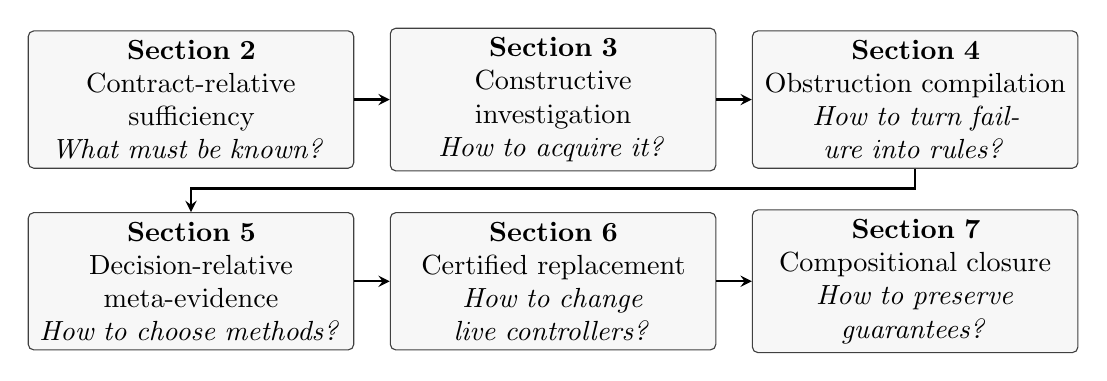
\begin{tikzpicture}[
    node distance=0.35cm and 0.45cm,
    box/.style={rectangle, draw=black!75, rounded corners=2pt, align=center,
                text width=3.9cm, minimum height=1.25cm, fill=black!3},
    arrow/.style={->, >=stealth, thick}
]
\node[box] (b1) {\textbf{Section 2}\\Contract-relative sufficiency\\\emph{What must be known?}};
\node[box, right=of b1] (b2) {\textbf{Section 3}\\Constructive investigation\\\emph{How to acquire it?}};
\node[box, right=of b2] (b3) {\textbf{Section 4}\\Obstruction compilation\\\emph{How to turn failure into rules?}};

\node[box, below=0.55cm of b1] (b4) {\textbf{Section 5}\\Decision-relative meta-evidence\\\emph{How to choose methods?}};
\node[box, right=of b4] (b5) {\textbf{Section 6}\\Certified replacement\\\emph{How to change live controllers?}};
\node[box, right=of b5] (b6) {\textbf{Section 7}\\Compositional closure\\\emph{How to preserve guarantees?}};

\draw[arrow] (b1) -- (b2);
\draw[arrow] (b2) -- (b3);
\draw[arrow] (b3.south) -- ++(0,-0.25) -| (b4.north);
\draw[arrow] (b4) -- (b5);
\draw[arrow] (b5) -- (b6);
\end{tikzpicture}
\caption{The conceptual progression of CRTT; arrows denote the progression of research questions, not necessarily source imports.}
\label{fig:arch-map}
\end{figure}

\begin{table}[h]
\centering
\footnotesize
\begin{tabular}{@{}p{3.6cm}p{5.2cm}p{4.6cm}@{}}
\toprule
\textbf{Established Result} & \textbf{Discovered Boundary} & \textbf{Next Object of Study} \\
\midrule
Functional replaceability & No valid operator may exist & Obstruction \\
Observation sufficiency & Required information is not known a priori & Observation strategy \\
Optimal strategy & Re-synthesis on new tasks is costly & Transfer \\
Transferability & A transfer morphism must be found & Constructive discovery \\
Complete discovery & Exhaustive search is too expensive & Certified pruning \\
Rule learning & Valid learning need not pay for itself & Meta-controller \\
Controller selection & Exact method costs are only partially known & Meta-evidence \\
Sufficient meta-evidence & Live replacement can break a continuation & Certified migration \\
Sound migration & Repeated changes interact across history & Compositional trace laws \\
Controller replacement & The selection policy itself may be inadequate & Meta-policy closure \\
\bottomrule
\end{tabular}
\caption{Research questions induced by the limits of preceding constructions.}
\label{tab:genesis}
\end{table}

\subsection{Reading Guide and Supplementary Archive}
Sections~\ref{sec:foundations}--\ref{sec:meta-evidence} build the constructive and economic machinery required to state and prove our central results in Sections~6 and~7. Full Lean~4.36.0 sources (21 canonical files, 542 audited declarations), historical gate records, and nine CLI execution witnesses are provided in the accompanying reconciled release archive (\texttt{CRTT-v1.0-FULL-ARCHITECTURE-RECONCILED.zip}), which serves as the formal supplementary material.

% ============================================================================
\section{Contract-Relative Foundations}
\label{sec:foundations}
% ============================================================================

\subsection{Contracts, Sufficiency, and the Existence Criterion}
Fix a state space $X$, a non-empty action space $A \neq \varnothing$, and a contract predicate $V : X \times A \to \mathrm{Prop}$. For each $x \in X$, define its set of contract-admissible actions $A_C(x) = \{ a \in A \mid V(x, a) \}$. An observation map $\phi : X \to Z$ induces a fiber $\phi^{-1}(z) = \{ x \in X \mid \phi(x) = z \}$ over each signature $z \in \phi(X)$. A total policy $\pi : Z \to A$ is \emph{contract-admissible through $\phi$} if $V(x, \pi(\phi(x)))$ holds for all $x \in X$.

\begin{theorem}[Contract-Relative Sufficiency Criterion (\texttt{CRTT.selector\_iff})]
\label{thm:sufficiency}
Assume $A \neq \varnothing$. An observation map $\phi : X \to Z$ admits a contract-admissible total policy $\pi : Z \to A$ if and only if every realized fiber admits a common admissible action:
\begin{equation}
\label{eq:sufficiency}
\exists \pi : Z \to A,\; \forall x \in X,\; V(x, \pi(\phi(x)))
\iff
\forall z \in \phi(X),\; \bigcap_{\phi(x) = z} A_C(x) \neq \varnothing.
\end{equation}
\end{theorem}

\begin{proof}
($\Rightarrow$) If $\pi$ satisfies $V(x, \pi(\phi(x)))$ for all $x$, then for any $z \in \phi(X)$, $\pi(z) \in \bigcap_{\phi(x)=z} A_C(x)$.
($\Leftarrow$) For each $z \in \phi(X)$, select a witness $a_z \in \bigcap_{\phi(x)=z} A_C(x)$ (using classical choice in the general setting). For $z \notin \phi(X)$, set $\pi(z) = a_0$ for an arbitrary $a_0 \in A$, which exists because $A \neq \varnothing$. The resulting total policy satisfies $V(x, \pi(\phi(x)))$ for all $x \in X$.
\end{proof}

Notice that without $A \neq \varnothing$, the criterion fails when $X = \varnothing$ and $Z \neq \varnothing$. Moreover, this early general result relies on classical choice, in sharp contrast to the constructive finite search in the canonical stack, whose audited declarations do not depend on \texttt{Classical.choice}.

\subsection{Collective Obstructions and Coarsest Partitions}
Criterion~\eqref{eq:sufficiency} shows that sufficiency fails whenever some fiber has empty admissible intersection. Crucially, refining $\phi$ cannot always resolve such an obstruction: if $A_C(x) = \varnothing$ for some $x \in X$, then even complete state observation admits no valid action.

Even when every individual state is solvable ($A_C(x) \neq \varnothing$), obstructions need not be pairwise. Define world compatibility by
\[
x \sim_C y \iff A_C(x) \cap A_C(y) \neq \varnothing.
\]
Consider three worlds with admissible action sets $A_C(x_1)=\{a,b\}$, $A_C(x_2)=\{b,c\}$, and $A_C(x_3)=\{a,c\}$ (\texttt{SufficientPartitions.triangle\_compat\_all}, \texttt{triangle\_no\_common\_action}). Every pair of worlds shares an admissible action, yet $\bigcap_{i=1}^3 A_C(x_i) = \varnothing$: the obstruction is strictly collective. This phenomenon constrains the existence of a greatest sufficient partition in the refinement order (not a minimum-size encoding).

\begin{theorem}[Existence of a coarsest sufficient partition]
\label{thm:coarsest}
A coarsest sufficient partition of $X$ exists if and only if $\sim_C$ is an equivalence relation and the partition induced by $\sim_C$ is itself sufficient.
\end{theorem}

\begin{proof}[Proof sketch]
If $\sim_C$ is a sufficient equivalence relation, any sufficient partition must place incompatible worlds in distinct classes, so it refines $\sim_C$; thus $\sim_C$ is coarsest. Conversely, suppose a coarsest sufficient partition $\mathcal{P}^*$ exists. Its sufficiency implies $A_C(w)\ne\varnothing$ for every $w$. Thus any compatible pair $x\sim_C y$ can be merged while all other states remain singleton blocks; since $\mathcal{P}^*$ is coarsened by every sufficient partition, $x$ and $y$ must lie in the same class of $\mathcal{P}^*$. On the other hand, sufficiency of $\mathcal{P}^*$ forces any two states in the same class to be compatible. Hence $\sim_C$ coincides with the equivalence relation of $\mathcal{P}^*$ and is sufficient.
\end{proof}

The corresponding declaration is \texttt{coarsest\_exists\_iff} in \texttt{SufficientPartitions.lean}. In the triangle example above, $\sim_C$ is the universal relation (hence an equivalence), but it is not sufficient; therefore no coarsest sufficient partition exists. In contrast, for an exact target $g:X\to Y$, equality of target values is itself the coarsest sufficient relation (\texttt{exact\_target\_coarsest}).

\subsection{Economic Foundations: Library Accumulation and Minimax Regret}
Once sufficiency is established, the economic analysis examines when accumulating methods or acquiring observations pays off under finite budgets:
\begin{itemize}
    \item \textbf{Idealized accumulation and strict gain:} For a fixed feasible trace predicate, with reuse no dearer than discovery and no additional lookup charge, budgeted reachability is monotone under library inclusion. Writing $C_{\mathrm{ind}}^*$ and $C_{\mathrm{cum}}^*$ for the attained minima over the same feasible plans, with $C_{\mathrm{ind}}(p)=C_{\mathrm{cum}}(p)+S(p)$ for every feasible $p$, strict cumulative gain holds if and only if some admissible plan $p$ yields certified savings $S(p)$ exceeding its independent suboptimality gap:
    \begin{equation}
    \label{eq:t15}
    C_{\mathrm{cum}}^* < C_{\mathrm{ind}}^* \iff \exists p :\; S(p) > C_{\mathrm{ind}}(p) - C_{\mathrm{ind}}^*.
    \end{equation}
    \item \textbf{Mandatory lookup costs and online thresholds:} Mandatory lookup charges can break monotonicity: a library extension increases cost from $2$ to $3$ at budget $2$. In the hidden-method model, an adversarial hidden repeated method yields regret $D-R$ for a deterministic first choice when discovery costs $D$, reuse costs $R\le D$, and at least two tasks occur. In the separate repeated-task threshold model with rent $L$ and $R<L\le D$, the break-even strategy is $2$-competitive against the offline optimum.
    \item \textbf{Minimax regret and value of observation:} On a finite list of scenarios and a nonempty finite action list, with decidable observation equality, let $c(a,x)\in\mathbb N$ and define action regret $r(a,x) = c(a,x) - \min_{b \in A} c(b,x)$ and the worst-case minimax regret of an observation map $\phi$ by
    \begin{equation}
    \label{eq:t18-regret}
    R^*(\phi) = \max_{z \in \phi(X)} \min_{a \in A} \max_{x : \phi(x)=z} r(a,x).
    \end{equation}
    The maximum of an empty scenario list is zero. The minimax criterion characterizes $\varepsilon$-sufficiency by existence of a common action with regret at most $\varepsilon$ in each realized fiber. In its XOR witness, no observation or either bit alone has regret $1$, whereas both bits give regret $0$. Acquiring a fixed refinement $\phi'$ at charge $c_{\mathrm{obs}}$ is strictly advantageous precisely when
    \begin{equation}
    \label{eq:t18-acq}
    c_{\mathrm{obs}} + R^*(\phi') < R^*(\phi).
    \end{equation}
\end{itemize}

\subsection{From sufficiency to investigation}
These results include an online threshold model but do not yet provide the general bounded-depth tree synthesizer and typed task-transfer mechanism developed below. This motivates the constructive investigation and transfer layer (Section~3).

The foundational results have separate historical proof artifacts. The self-contained canonical stack establishes the release theorem independently of those branches; Section~8 records their provenance.

\clearpage
\section{Constructive investigation and transfer}\label{sec:investigation}
Sufficiency gives a criterion for a fixed observation but not an acquisition strategy. We first synthesize finite adaptive investigations, then ask when an already synthesized strategy can be transported to another task. The declared world, action and port lists are finite; equality of ports is decidable. No efficiency bound on exhaustive synthesis is asserted.

\subsection{Adaptive investigation synthesis}
A task has a declared list of worlds $E$, a nonempty action list $\mathcal A$, a port list $Q$, a read function $r(q,w)\in\{0,1\}$, port prices $c(q)\in\Nat$, terminal losses $L(a,w)\in\Nat$, and depth limit $d$. An investigation is a finite tree
\[
 t ::= \operatorname{act}(a)\mid\operatorname{observe}(q,t_0,t_1).
\]
Legality requires declared actions and ports, depth at most $d$, and no repeated port along a path (all occurrences of a purchased port are removed from the remaining list). With $J_w(t)$ its realized cost, the semantics is $J_w(\operatorname{act}(a))=L(a,w)$ and $J_w(\operatorname{observe}(q,t_0,t_1))=c(q)+J_w(t_{r(q,w)})$. Only the realized branch is charged. Let $W_E(t)=\max_{w\in E}J_w(t)$, with empty maximum zero, and $V_d(E,Q)$ be the optimal legal worst cost. Write $E_b(q)$ for the filter of $E$ with read value $b$ and $L_*(E)=\min_{a\in\mathcal A}\max_{w\in E}L(a,w)$.

\begin{theorem}[Optimal finite investigation]\label{thm:investigation}
The executable solver attains $V_d(E,Q)$ with a legal tree. For $E\ne\varnothing$,
\begin{align}
 V_0(E,Q)&=L_*(E),\\
 V_{d+1}(E,Q)&=\min\Bigl(\{L_*(E)\}\cup\{c(q)+\max_{b\in\{0,1\}} \\
 &\hspace{24mm} V_d(E_b(q),Q\setminus\{q\}):q\in Q\}\Bigr).
\end{align}
For empty $E$ the value is zero. For a hard terminal tolerance $\epsilon$ and observation budget $b$, replace terminal loss by $0$ when $L(a,w)\le\epsilon$ and by $b+1$ otherwise. The capped optimum is at most $b$ if and only if a legal tree meets both bounds on every declared world.
\end{theorem}
\begin{proof}
Induct on depth. Every legal tree is a terminal action or starts with a declared port and two legal subtrees at smaller depth. For nonempty $E$, the worst observation-node cost is the fee plus the maximum of the two branch costs, since one branch is realized and all costs are nonnegative. The solver chooses the least-cost candidate among the terminal optimizer and recursively synthesized observation candidates. By induction every competing tree has cost at least this minimum, and the chosen candidate is legal. In the capped problem a violating terminal leaf costs at least $b+1$; a valid leaf contributes zero, so the worst cap is precisely the hard feasibility test. See \rc{solve\_legal}, \rc{solve\_optimal}, \rc{bellman}, and \rc{epsilon\_budget\_iff} in \rc{AdaptiveObservation.lean}.
\end{proof}
The adaptive optimum is at most the best legal fixed-schedule value (\rc{adaptive\_le\_static}). The multiplexer witness reads a selector bit then the indicated data bit, attaining cost $2$ rather than the static optimum $3$ under unit prices and wrong-answer loss $4$. The XOR witness also excludes a general greedy one-step value rule. Synthesis here is exact within the declared tree language, not over arbitrary programs.

\subsection{Transport and library economics}
For tasks $S,T$, a transfer morphism $M=(h,p,a)$ maps target worlds to source worlds, source ports to target ports, and source actions to target actions, preserving declared membership. The port map is injective on declared source ports, $d_S\le d_T$, and for all declared arguments
\begin{align*}
 r_T(p(q),w)&=r_S(q,h(w)), & c_T(p(q))&\le c_S(q),\\
 L_T(a(u),w)&\le L_S(u,h(w)).
\end{align*}
Transport $M_*t$ is the syntax-directed substitution of port and action labels, independent of the unknown target world.
\begin{theorem}[Certified transfer]\label{thm:transfer}
For every source-legal tree $t$, $M_*t$ is target-legal and $J^T_w(M_*t)\le J^S_{h(w)}(t)$ for every declared target world. Observation charges and terminal losses are separately nonincreasing. Hence $V_T\le V_S$; mutual morphisms imply equality of optima. Identity and composition of morphisms induce identity and composition of tree transports.
\end{theorem}
\begin{proof}
Structural induction on the tree gives corresponding branch choices by read equality and the cost inequalities by addition; injectivity ensures removal of an observed port cannot remove a different source port's image. The depth inequality gives legality. Maximizing over target worlds and applying the result to a source optimizer proves the value inequality. Composition is function composition (contravariant on worlds) and tree substitution composes. These are the \rc{transfer\_legal}, \rc{transfer\_runCost\_le}, \rc{transfer\_hard\_contract}, \rc{optimum\_le}, \rc{mutual\_optimum\_eq}, and \rc{transfer\_compose} results of \rc{InvestigationTransfer.lean}.
\end{proof}
Equal optimum values alone do not imply the existence of a morphism; the finite equal-optimum witnesses show failures of injectivity and of loss preservation. Moreover, transport incurs fees. For a listed route with overhead $k$ and target execution cost $e\ge V_T$, reuse is strictly cheaper than fresh synthesis at charge $D$ followed by optimal execution exactly when $k+(e-V_T)<D$. The explicit library selector minimizes over the fresh option and listed certified offers; with search charge $s$ and fresh quote $F$, search pays off iff some discovered offer has $s+k+e<F$. Completeness relative to the semantic offer oracle requires a cost-complete admitted list, not merely a sound subset. These are \rc{paid\_candidate\_iff}, \rc{search\_profitable\_iff}, and \rc{complete\_search\_matches\_oracle} in \rc{InvestigationLibrary.lean}.

\subsection{Constructive discovery of morphisms}
A transfer theorem is useful only once its witness is available. For indexed finite tasks (all actions declared, including a default action), enumerate all maps $p:Q_S\to Q_T$ and $a:\mathcal A_S\to\mathcal A_T$. For a fixed pair define
\[
 \mathcal Y_w(p,a)=\{y\in X_S: \forall q\in Q_S,\ r_T(p(q),w)=r_S(q,y),\quad
 \forall u\in\mathcal A_S,\ L_T(a(u),w)\le L_S(u,y)\}.
\]
\begin{theorem}[Canonical discovery]\label{thm:discovery}
A fixed pair $(p,a)$ extends to a morphism iff the depth and port conditions hold and $\mathcal Y_w(p,a)\ne\varnothing$ for every target world $w$. Picking the first witness in each finite source row constructs a morphism. The list $\CanonRef=\rc{discoverAll}(S,T)$ contains a representative with the same port and action maps as every valid morphism; it is empty iff no morphism exists.
\end{theorem}
\begin{proof}
A valid world map supplies a member of each row. Conversely, each target world can be assigned its first row member independently, since the morphism has no inter-world constraints. This establishes all read and loss obligations, while the separately checked depth, price and injectivity obligations are unaffected. Exhaustive map enumeration supplies the pair of any valid morphism. A nonempty output itself inhabits the morphism type. See \rc{fixed\_pair\_iff}, \rc{discover\_complete}, and \rc{empty\_iff\_no\_morphism} in \rc{MorphismDiscovery.lean}.
\end{proof}
The canonical list need not enumerate all possible world maps; the translated tree depends only on $p,a$. This removes exhaustive enumeration of global world maps, not the potentially expensive enumeration of the remaining pairs. The next problem is how to preserve this reference semantics under interruption, pruning, and learning.

\clearpage
\section{Budgeted discovery and obstruction compilation}\label{sec:obstruction}
The finite reference list $\CanonRef$ specifies what discovery must recover; computing it in advance would defeat the purpose of a budgeted search. We use a paid executor whose correctness is stated against $\CanonRef$ without calling the reference enumeration at each step.

\subsection{Paid prefixes and certified pruning}
A deterministic quote maps a state $u$ to no step or a pair $(\eta, k)$ with positive natural charge $\eta$ and delayed successor $k:\mathrm{Unit}\to U$. The account is $(u,B,D)$ with remaining balance $B$ and recorded spend $D$. If $\eta\le B$ the executor invokes the successor and changes the account to $(k(),B-\eta,D+\eta)$; otherwise it stops without invoking it. The bounded run counts steps separately from money, and execution with fuel $B$ suffices to reach a state with no affordable next step. Induction gives exact conservation $B'+D'=B+D$ and preservation of any inductive invariant of quoted transitions (\rc{accounting}, \rc{invariant}, \rc{budget\_bound} in \rc{BudgetedDiscovery.lean}).

\begin{theorem}[Exact budget continuation]\label{thm:resume}
For a fixed, budget-independent deterministic quote with positive charges, let $\mathsf E$ be the executor and $\mathsf U_b$ add $b$ to the account balance. Then
\[
 \mathsf E\mathsf U_{b_1+b_2}(s)=\mathsf E\mathsf U_{b_2}(\mathsf E\mathsf U_{b_1}(s)).
\]
This equality includes the state, balance and spend, even for a cyclic underlying transition system.
\end{theorem}
\begin{proof}
Each affordable prefix under the smaller budget is also affordable under the larger one; payment commutes with adding the difference. Apply induction to the paid prefix, with the nonpayable and absent-step cases stationary. Positive charges bound the number of paid steps by the balance, giving the saturated-executor identity. This is \rc{execute\_topUp\_add} in \rc{ResumeLaws.lean}. The theorem does not imply semantic exhaustion; a loop may simply consume its budget.
\end{proof}
In the morphism search, a partial port assignment $\rho$ denotes the region of morphisms extending it. A certified pruning rule consists of a Boolean test $k(\rho)$, a charge, and the witness
\[
 \forall M,\rho,\quad \operatorname{Extends}(M,\rho)\Longrightarrow k(\rho)=\mathrm{true}.
\]
A false result excludes the entire region. Rules may test injectivity, port prices, depth or read compatibility, and sound rules can be composed. The pruned search uses the same canonical pair constructor as Section~3.

\begin{theorem}[Pruning preserves canonical membership]\label{thm:prune}
For every certified rule and morphism $x$, membership in the resulting exhaustive pruned list is equivalent to $x\in\CanonRef$.
\end{theorem}
\begin{proof}
A retained complete assignment is checked by the reference pair constructor, giving soundness. For completeness, follow the prefixes of any canonical representative's port map; soundness of each rule ensures every such prefix survives. The reference action map is then considered and yields the same canonical certificate. This is \rc{prunedDiscover\_iff} in \rc{CertifiedPruning.lean}; no equality of list order or multiplicity is required.
\end{proof}
Sound pruning need not save resources: for $n_1\le n_0$ visited nodes, uniform node charge $c$ and per-node rule charge $k$, it pays precisely when $n_1 k<(n_0-n_1)c$ (\rc{pruning\_profitable\_iff}). A sound no-op rule increases cost if it is charged. The richer executor below accounts for actual short-circuit rule calls separately.

\subsection{A funded search frontier}
The frontier $f=(J,A,\Lambda)$ contains remaining jobs $J$, emitted canonical certificates $A$ and paid search receipts $\Lambda$. A job either extends a port-assignment region with its remaining rule queue or processes a remaining action-map suffix. A correct frontier contains only canonical certificates and covers every canonical certificate not yet emitted by at least one remaining job; see the exact predicate in Section~6.1. Splitting a job, rejecting a certified region, or checking a pair preserves this predicate and appends any new certificate. The proof uses local coverage and soundness, not a run of the reference enumeration.

Let $P(C,f)$ be the natural-number remaining-liability potential for a fixed rule library and base fees. Its job budgets bound the full branching work, including rule charges. Every quoted paid step satisfies
\begin{equation}\label{eq:funded-potential}
 P(C,f')+\eta\le P(C,f),\qquad\eta>0.
\end{equation}
\begin{theorem}[Funded exhaustion]\label{thm:funded-search}
Starting from a correct frontier with $B\ge P(C,f)$, the executor exhausts its jobs, preserves prior certificates as a list prefix, and returns a list whose membership is exactly $\CanonRef$. An empty exhausted certificate list proves nonexistence of a morphism.
\end{theorem}
\begin{proof}
Equation~\eqref{eq:funded-potential} preserves funding after payment and strictly decreases the potential. At quiescence a pending job would have an affordable positive quote, contradicting quiescence. Local correctness is inductive, and empty jobs eliminate the remaining-coverage disjunct. Prefix preservation follows by induction on append-only certificate emission. These are \rc{quote\_potential}, \rc{execute\_funded\_exhausts}, \rc{execute\_full}, \rc{execute\_certificate\_prefix} and \rc{exhausted\_impossible} in \rc{BudgetedPruning.lean}.
\end{proof}
Without the funding hypothesis the classifier distinguishes a found witness, an empty exhausted frontier with impossibility proof, and an inconclusive empty nonexhausted frontier. Its returned account supports continuation. A found witness before exhaustion is not a claim of enumeration completeness.

\subsection{From a failed row to a reusable rule}
For a target world $w$, a partial port assignment $\rho$ defines the read-compatible row
\[
 Y_w(\rho)=\{y\in X_S: \forall(q,q')\in\rho,\ r_S(q,y)=r_T(q',w)\}.
\]
If $Y_w(\rho)=\varnothing$, adding constraints cannot restore a member. The obstruction compiler deletes constraints while retaining an empty row, producing a subset $K\subseteq\rho$ that remains bad but becomes nonbad on deletion of any of its constraint values. Thus $K$ is irreducible by inclusion, not necessarily of minimum cardinality.
\begin{theorem}[Certified obstruction compilation]\label{thm:core}
Given an empty read row, \rc{extract} constructs such an irreducible $K$ with its witness. Every assignment containing $K$ admits no extending morphism. The compiled test rejects precisely assignments containing $K$ and satisfies the certified-rule contract.
\end{theorem}
\begin{proof}
The shrink procedure scans the original constraints, removing a value if badness persists. If removal fails, monotonicity of badness ensures that later deletions cannot make that removal bad again. The retained subset is therefore irreducible. If an extending morphism existed for an assignment containing $K$, its world map at $w$ would give a member of the empty row. The Boolean containment test is exact by membership reflection. See \rc{shrink\_spec}, \rc{extract}, \rc{core\_excludes}, \rc{compileCore\_rejects} in \rc{ImpasseCompilation.lean}.
\end{proof}
Core transport to a new task pair is permitted with a constraint map, a new-to-old source-world map, and a read-reflection proof on every translated constraint (\rc{transportCore}); irreducibility and economic superiority of the transported rule are not guaranteed.

The learning executor makes this compilation endogenous. The search state includes an active core library, raw and reduced learned events, pending compilation, and paid receipts. Lookup, probing, compilation, and base search advancement are distinct positive-charge transitions. A core is inserted with subsumption: if an old core already excludes all of its region, it is not installed; otherwise cores whose constraints contain the new core are removed. The resulting rejected region is exactly the union of the old rejection region and the new core's region (\rc{insertCore\_rejects}); past learned events remain in the history. Theorems \rc{execute\_correct}, \rc{execute\_trace}, \rc{execute\_split}, and \rc{execute\_exhausted\_iff} in \rc{LearningDiscovery.lean} preserve the semantic and accounting guarantees. Exhaustion is conditional, not guaranteed by arbitrary learning allowances.

This construction makes negative results operationally reusable. It does not establish a universally cheaper learner. In the declared finite stand, learning cost more than the fixed read-rule controller in all 515 fully completed cases. The next problem is therefore selection of the investigative mechanism itself, rather than unconditional learning.

\clearpage
\section{Decision-relative meta-evidence}\label{sec:meta-evidence}
A certificate of correct learning is not a certificate of economic gain. We now distinguish the cost of selecting a controller, the cost of learning about its cost, and the sufficiency of that evidence for a decision. The finite meta-problem is itself an instance of the investigation model of Section~3; its scenarios are task pairs of fixed carrier sizes.

\subsection{Selecting funded investigative plans}
A plan specifies a base rule-schema list, a learning allowance $\lambda$, a completion reserve $R$, and setup charge $k$. It first runs the paid learning prefix within $\lambda$, then hands the current frontier and unspent allowance plus $R$ to a static pruning executor. A proof that this handoff balance dominates the static liability potential is required. The prefix record, including any pending learning event, is returned separately; pending compilation is not a remaining answer obligation. With zero allowance the learning phase is disabled, including its lookup charges.

\begin{theorem}[Funded plans and meta-selection]\label{thm:meta-selection}
Each funded plan returns precisely the canonical membership of its task pair. Its actual modeled bill, including setup, is at most $k+\lambda+R$. For a finite catalogue of such plans indexed by actions, suppose a table $U(a,w)$ bounds the actual completed bill $C(a,w)$ for every plan and scenario, and a fixed controller fee $k_0$ is declared. The investigation optimizer of Section~3 minimizes $k_0+W_E(t)$ for terminal loss $U$; its predicted worst bill bounds actual execution. If $U=C$ everywhere, the optimizer minimizes actual worst bill over legal meta-trees.
\end{theorem}
\begin{proof}
The learning prefix preserves correctness. The funded handoff completes by Theorem~\ref{thm:funded-search}; conservation across the two phases gives the bound and keeps unspent reserve distinct from expenditure. At the meta-level the chosen tree executes only its selected plan. For each world its actual cost is the sum of realized query fees and $C(a,w)$, bounded by the corresponding sum using $U$. Theorem~\ref{thm:investigation} optimizes this upper objective; exactness of the table converts the inequality to actual optimality. See \rc{perform\_complete}, \rc{actualBill\_le\_reservation}, \rc{optimizer\_bound\_optimal} and \rc{optimizer\_actual\_optimal} in \rc{MetaInvestigation.lean}.
\end{proof}
The table, funding proofs and controller fee are supplied, not inferred from an unpaid oracle. An explicit witness reduces the worst modeled bill from $53$ to $25$ (including the declared meta-observation fee); the offline full-table acquisition costs $465$. With these fixed charges, strict amortization requires at least $17$ uses, since $465+25n<53n$ iff $465<28n$. This is a modeled witness, not a prediction of future workload. The need to acquire the cost table motivates partial evidence.

\subsection{Interval evidence and paid refinement}
For fixed worlds, ports, prices and depth, each unknown terminal cost $C(a,w)$ is represented by a proof-indexed interval
\[
  L(a,w)\le C(a,w)\le U(a,w).
\]
Intervals may be intersected; lower endpoints rise, upper endpoints fall, and the actual cost remains covered. Let $V_L,V_C,V_U$ denote the respective minimax values, $W_C$ the worst cost under actual losses, and $t_U$ an optimizer of the upper model.
\begin{theorem}[Sufficient interval certificate]\label{thm:interval}
$V_L\le V_C\le V_U$, and for every legal competing tree $t$,
\[
 W_C(t_U)\le W_C(t)+(V_U-V_L).
\]
The gap $V_U-V_L$ cannot increase under interval refinement. In particular, a gap at most $\epsilon$ suffices to certify the upper optimizer as $\epsilon$-near-optimal relative to the actual minimax objective.
\end{theorem}
\begin{proof}
Tree costs are monotone in terminal losses, and legality is unchanged, so the corresponding optimal values are ordered. Then $W_C(t_U)\le V_U\le W_C(t)+V_U-V_L$, using $V_L\le V_C\le W_C(t)$. Refinement improves both endpoints in the appropriate directions. The formal statements are \rc{lower\_le\_true}, \rc{true\_le\_upper}, \rc{certified\_gap}, and \rc{gap\_monotone} in \rc{MetaEvidenceAcquisition.lean}.
\end{proof}
Acquisition and assessment are separate positive-charge operations in a supplied finite schedule. The actual-indexed bound is acquired only after paying its quoted charge; the runner records fees, updates evidence monotonically and stops upon a sufficient certificate or budget/schedule exhaustion. The theorem \rc{assess\_complete} is completeness of the gap test, not a necessary condition for near-optimality. For the specific funded-plan family, acquiring six of eight exact cells certifies value $22$ at prepaid charge $2309$, compared with $3051$ for full acquisition; this is an ex-post schedule witness, not an optimal acquisition algorithm. Reserve-based prepaid charge is not identical to realized experimental cost.

\subsection{Decision sufficiency and optimal evidence acquisition}
Cost uncertainty does not imply decision uncertainty. For example, in two possible models with costs $(0,1)$ and $(100,101)$ for the same two controllers, the first is optimal in both despite a wide range of optimal values. We therefore use a finite nonempty catalogue $\mathcal C$ of admitted controllers and a list $E$ of compatible hypotheses. Each hypothesis $h$ has a bill $J_h(c)$ and reference $v_h\le J_h(c)$ for all $c\in\mathcal C$. The reference can be the attained catalogue minimum, but need not be the optimum over any larger class. Define
\[
 r_h(c)=J_h(c)-v_h,\qquad R(E)=\min_{c\in\mathcal C}\max_{h\in E}r_h(c),
\]
with empty maximum zero.
\begin{theorem}[Decision-relative sufficiency]\label{thm:decision}
$R(E)\le\epsilon$ iff some admitted controller satisfies $J_h(c)\le v_h+\epsilon$ for every $h\in E$. For the catalogue reference this is equivalently $J_h(c)\le J_h(c')+\epsilon$ for all $h\in E,c'\in\mathcal C$. Refining the hypothesis list cannot increase $R$.
\end{theorem}
\begin{proof}
The minimum is attained by finite selection, and the maximum bound is equivalent to the pointwise inequalities. For the catalogue case, one direction uses the lower bound of the catalogue minimum on all competitors, and the converse uses an attaining competitor for each hypothesis. Subset refinement can only reduce each controller's worst regret, hence the minimum. These are \rc{residual\_iff}, \rc{catalogue\_robust\_iff}, and \rc{residual\_subset} in \rc{DecisionEvidence.lean}.
\end{proof}
Pairwise bounds on costs can certify this decision without identifying the cost model. Exact hypothesis membership is an explicit external premise: a deterministic response to a port $q$ filters $E$, preserving the actual hypothesis if it was present initially (\rc{refine\_truth}). Taking terminal loss $r_h(c)$ in the investigation model produces the optimal acquisition tree for worst-case query expenditure plus regret, with terminal value $R(E)$ and the Bellman recurrence of Section~3. This is \rc{acquisition\_optimal} and \rc{acquisition\_bellman}. The actual total bill, for external setup $k$, is exactly $k+v_h+$ realized query-plus-regret cost; minimizing worst regret is not in general minimizing worst actual bill when $v_h$ varies (\rc{total\_bill\_identity}).

A hard contract is different from the soft sum. Using the capped construction of Theorem~\ref{thm:investigation}, \rc{hardAssess} succeeds iff a legal acquisition tree exists with observation expenditure at most $b$ and terminal regret at most $\epsilon$ on every compatible hypothesis. Whenever feasible, its tree also minimizes worst observation expenditure among legal trees satisfying the regret tolerance (\rc{hard\_assess\_complete}, \rc{hard\_minimal\_observation}). These guarantees require actual membership and a specified finite catalogue, not automatic hypothesis generation or free validation. In particular, selecting a controller prospectively does not authorize its installation into a partially explored live frontier. That is the separate replacement problem of Section~6.

\clearpage
\section{Certified controller replacement}\label{sec:replacement}
The preceding constructions separate the existence of a transferable investigation from the cost of finding it. Selecting a controller before a search begins, however, does not justify replacing that controller during a partially completed search. A replacement must preserve the unresolved obligations as well as the results already certified, and it must be possible to pay for the change without losing the ability to finish. We now fix the indexed source and target tasks $S,T$ and the canonical reference list $\CanonRef=\rc{discoverAll}(S,T)$ of Section~3. Throughout Sections~6--7, resource-accounting quantities denote natural-number model charges, not measured time or memory.

\subsection{Continuations and their denotation}
A controller $C=(\mathcal R,\tau)$ consists of a certified pruning-rule library and base search tariffs. A frontier $f=(J,A,\Lambda)$ contains pending jobs $J$, a list of certified morphisms $A$, and a list of search receipts $\Lambda$. Writing $\Cov(x,J)$ for coverage of a morphism by a pending job, frontier correctness is exactly
\begin{equation}\label{eq:frontier-correct}
 \Correct(f)\;\Longleftrightarrow\;
 (A\subseteq\CanonRef)\ \land\
 \bigl(\forall x\in\CanonRef,\ x\in A\ \lor\ \Cov(x,J)\bigr),
\end{equation}
where inclusion and membership concern lists, not an assertion of uniqueness or disjointness. The frontier thus represents both established knowledge and remaining search obligations. For frontiers $f,g$ define continuation equivalence by
\begin{equation}\label{eq:same-cont}
 f\simeq g\;\Longleftrightarrow\;
 A_g=A_f\ \land\ \Lambda_g=\Lambda_f\ \land\
 \forall x:\mathrm{Morphism}(S,T),\ \Cov(x,J_g)\leftrightarrow\Cov(x,J_f).
\end{equation}
A continuation $c=(C,f,R;\pi)$ contains a proof $\pi$ of correctness and of the potential bound $P(C,f)\le R$. The reserve $R$ is a sufficient upper bound on completion resources, not an expenditure. Define $b(c)=\bill(c)$ to be the actual modeled bill of running the current static continuation to exhaustion from balance $R$ and zero incremental spend. By funded completion, $b(c)\le R$. A live state also requires $R\le B$, where $B$ is its available balance.

\begin{theorem}[Continuation-preserving replacement]\label{thm:rebase}
Replacing $\mathcal R$ by another certified library $\mathcal R'$ with the same $\tau$, rebasing pending rule queues, and supplying a valid new reserve produces a continuation $c'$ with $f\simeq f'$. Its completion has exactly the same canonical membership as the completion of $c$; both have membership equal to $\CanonRef$.
\end{theorem}
\begin{proof}
The rebase operation resets only the rule queue of a pending port-region job. It leaves its region, every action job and its unprocessed suffix unchanged, and copies $A,\Lambda$ exactly. Coverage is independent of the rule queue, so coverage of every job, hence of their list, is invariant. Equation~\eqref{eq:same-cont} follows, and \eqref{eq:frontier-correct} transfers to the new frontier. Funded completion for each continuation gives membership in $\CanonRef$ independently of the selected rule library. These are \rc{rebase\_same}, \rc{same\_correct}, and \rc{completion\_full} in \rc{ControllerReplacement.lean}.
\end{proof}
This equivalence is stronger than equality of final answer sets: it preserves the outstanding denotation without restarting the search. It does not authorize arbitrary executable-code migration or the transfer of a full learning state.

\subsection{Liquidity and comparative cost evidence}
An absolute offer is indexed by the exact incumbent $c$ and contains a new controller, same-fee and funding proofs, a migration charge $K$, and proved bounds $L\le b(c)$ and $b(c')\le U$. Let $H$ be the check charge. The numerical gate admits the offer if and only if
\begin{equation}\label{eq:absolute-gate}
 H+R\le B,\qquad H+K+R'\le B,\qquad H+K+U<L.
\end{equation}
The first inequality protects incumbent completion even if validation fails. The second protects completion after migration. The last establishes strict improvement, including the charges for both check and migration. A low remaining bill does not imply an affordable change, since the reserve is distinct from the bill.

Independent endpoints can discard decisive correlations. The relative-evidence construction therefore replaces a single pair $(L,U)$ by a finite list $E$ of paired lower and upper bounds with a supplied actual-pair coverage proof:
\begin{equation}\label{eq:actual-coverage}
 \exists (\ell,u)\in E:\quad \ell\le b(c)\quad\land\quad b(c')\le u.
\end{equation}
This is a joint certificate, not a list of unrelated marginal bounds. In particular, $E$ cannot be empty at the typed boundary, even though the raw universal arithmetic test would pass the empty list. The cost predicate is
\begin{equation}\label{eq:relative-gate}
 \operatorname{relativeOK}(H+K,E)\;\Longleftrightarrow\;
 \forall(\ell,u)\in E,\ H+K+u<\ell.
\end{equation}
For a singleton list $[(L,U)]$, this recovers the absolute economic test in \eqref{eq:absolute-gate}. For example, the paired rows $(7,1)$ and $(70,64)$ pass with $H+K=2$, whereas independent extrema $(7,64)$ fail. The second row in the release fixture represents synthetic uncertainty, not a measured second world.

\begin{theorem}[Exact admission and sound gain]\label{thm:gate}
For a typed relative offer, the fixed numerical gate returns \emph{accepted} if and only if the first two inequalities of \eqref{eq:absolute-gate} and \eqref{eq:relative-gate} hold. If accepted, $H+K+b(c')<b(c)$. Its application preserves continuation equivalence, base search tariffs and a funded reserve.
\end{theorem}
\begin{proof}
The equivalence is by the successive branches of \rc{gate}; the universal row test is reflected into a Boolean by \rc{relativeOK\_iff}. Choose the covering pair of \eqref{eq:actual-coverage}. Then $H+K+b(c')\le H+K+u<\ell\le b(c)$, which proves the strict gain. Rebasing uses Theorem~\ref{thm:rebase}. The accepted balance $B-H-K$ is at least $R'$ by the second guard. For rejection the incumbent is retained, and the first guard bounds its reserve by the post-check balance. For deferral the state is unchanged. These are \rc{gate\_accepted\_iff}, \rc{relative\_sound}, \rc{apply\_same}, and \rc{apply\_liquid}.
\end{proof}

The public attempt uses $H=h+1$ for a base charge $h\in\Nat$. Its verdict is an ordinary four-valued result; application requires a proof that this verdict is the output of the fixed gate on this exact state and offer. Table~\ref{tab:debit} gives the operational accounting. The first failed guard determines the verdict, and the row test is evaluated only after both reserve guards pass.
\begin{table}[htbp]
\centering\small
\caption{Admission accounting. $d$ is the debit, not the completion reserve.}\label{tab:debit}
\begin{tabularx}{\linewidth}{@{}lXll@{}}\toprule
Verdict & Condition (in order) & Installed & $d$\\\midrule
Deferred & Incumbent guard fails & $c$ & $0$\\
Reject liquidity & New reserve guard fails & $c$ & $H$\\
Reject gain & Paired gain test fails & $c$ & $H$\\
Accepted & All three tests pass & $c'$ & $H+K$\\\bottomrule
\end{tabularx}
\end{table}

Let a session $s$ contain the live state and a relative journal. Write $D(s)=\spent(s)$ for the sum of search receipts, legacy attempt charges, and relative journal charges, and $W(s)=B(s)+D(s)$ for the total funds. Application subtracts precisely $d$ from balance and adds $d$ to the ledger, preserving $W$. The proposal is already proof-bearing; the gate neither estimates the unknown bills by free prospective runs nor performs a proof search. It verifies the declared numerical conditions. External evidence charges record expenditure and do not by themselves certify the truth or acquisition of evidence.

\subsection{A law for mixed replacement histories}
For a funded session define the completion objective
\begin{equation}\label{eq:root-objective}
 \Phi(s)=D(s)+b(c_s).
\end{equation}
It is the total modeled spend obtained by finishing the incumbent, not an online estimate. Allowed actions are a funded prefix of the current search, an attempt indexed by the current continuation, and an affordable external evidence receipt. A connected trace $s_0\to\cdots\to s_n$ consists of actual action applications, with equality of adjacent endpoints; it is not a list of freely asserted postconditions. In particular no decidable equality of arbitrary function-bearing states is assumed.

For each step define its net gain $g_i$ and overhead $o_i$ as follows. An accepted replacement has $g_i=\Phi(s_{i-1})-\Phi(s_i)>0$, already net of check and migration, and $o_i=0$. A paid rejection or evidence charge has $g_i=0$ and $o_i$ equal to its charge. A search prefix or deferral has both zero. Let $G=\sum_i g_i$, $O=\sum_i o_i$, $N_p$ the number of non-deferred replacement attempts, and $N_a$ the number accepted.

\begin{theorem}[Compositional root accounting]\label{thm:root-trace}
For every connected finite root trace,
\begin{align}
 \Phi(s_n)+G&=\Phi(s_0)+O,\label{eq:trace-objective}\\
 W(s_n)&=W(s_0),& R(s_n)&\le B(s_n),\label{eq:trace-funds}\\
 N_p+B(s_n)&\le B(s_0),& N_a&\le G.
\end{align}
Moreover the endpoint relation $\Pres(s_0,s_n)$ preserves base search tariffs and the legacy attempt history exactly, the certificate list as a prefix, and search receipts and relative journal as suffixes of their reverse-chronological lists.
\end{theorem}
\begin{proof}
For a prefix of the fixed controller, deterministic continuation gives $b(c)=d+b(c')$, where $d$ is prefix spend. Thus \eqref{eq:root-objective} is unchanged. A deferred attempt is identity. A rejected attempt or an evidence receipt retains $c$ and increases $D$ by its recorded charge. Acceptance strictly decreases $\Phi$ by Theorem~\ref{thm:gate}; this difference defines its net gain. Every step consequently satisfies $\Phi(s_i)+g_i=\Phi(s_{i-1})+o_i$, conservation, and the indicated history relation. The certificate-prefix and receipt-suffix relations compose by list concatenation. Induct on the connected trace, adding both nonnegative statistics at each step; positive check tariffs bound the paid count, and each accepted gain is at least one. The identities are \rc{remainingBill\_prefix}, \rc{action\_laws}, \rc{laws\_compose}, and \rc{trace\_laws} in \rc{RecursiveTrace.lean}.
\end{proof}
Since $D(\finish(s))=\Phi(s)$, \eqref{eq:trace-objective} gives the necessary and sufficient condition for a strict net saving over immediate incumbent completion:
\begin{equation}\label{eq:net-gain}
 D(\finish(s_n))<D(\finish(s_0))\quad\Longleftrightarrow\quad O<G.
\end{equation}
This is \rc{trace\_final\_gain\_iff}. The theorem permits losses from exploratory attempts without weakening correctness. It also identifies the next obstruction: choosing when to incur such attempts can itself be inadequate. This motivates making the proposal policy an explicit, replaceable object rather than imposing a fixed sequence of heuristic interventions.

\section{Compositional meta-policy closure}\label{sec:closure}
\subsection{A paid and replaceable policy}
We now distinguish a root controller from the finite policy that decides whether to attempt its replacement. Fix an incumbent continuation $c_*$ and a provider $p$ indexed by $S,T,c_*$. The provider contains a deterministic Boolean observation thunk, a thunk returning a typed relative offer for $c_*$, and declared base charges for observing, preparing, and checking. A frame $f$ contains a session $s$ with a proof that $c_s=c_*$. A policy $t$ is a finite tree with leaves \emph{keep} or \emph{attempt}, and binary observation nodes. The concrete language uses a single observation port and permits repeated probes; it need not belong to the one-use legal tree class of the earlier optimal synthesis problem.

Interpretation is by structural recursion. A probe and preparation are invoked only in their funded branches, after the corresponding charge $h+1$ is posted while retaining the root reserve. A terminal attempt prepares an offer and invokes the fixed relative gate of Section~\ref{sec:replacement}; a failed guard blocks the relevant operation. Interpretation records actual Boolean responses, prepared typed offers, and verdicts. It produces a session $I_p(t,f)$ with preserved history and funds, regardless of whether a replacement was accepted. The policy is then completed by the funded root runner. Define its all-in bill (including already incurred expenditure) by
\begin{equation}\label{eq:policy-bill}
 \PB_p(t,f)=\Phi(I_p(t,f))=D(\finish(I_p(t,f))).
\end{equation}
The corresponding definitions and laws are in \rc{MetaPolicy.lean}. In particular, \rc{policyBill\_complete} proves the second equality.

A machine $m=(f,t,L)$ adds the current policy and its paid upgrade history $L$ to the frame. Consider a proposed replacement $t'$ with base setup charge $a$ and $q=a+1$. Before invoking the proposal factory, the upgrade operation checks $q+R\le B$. If this fails it returns the identical machine, without a charge or invocation. Otherwise it pays $q$, giving a new frame $f^+$ with the same incumbent, and invokes the factory. The supplied proposal proves
\begin{equation}\label{eq:policy-bounds}
 \lambda\le\PB_p(t,f),\qquad \PB_p(t',f^+)\le\upsilon.
\end{equation}
The fixed upgrade gate installs $t'$ exactly when $\upsilon<\lambda$, otherwise retains $t$ at $f^+$. Both paid outcomes record the prior and candidate tree, bounds and charge. The setup cost is already included by the post-payment frame in \eqref{eq:policy-bounds}; adding it again would double count. The provider and root contract do not change.

\begin{theorem}[Local policy improvement]\label{thm:policy-local}
Every executed upgrade preserves $W$, $\Pres$, liquidity, and prior upgrade history. An accepted upgrade from $m$ to $m'$ strictly decreases $\PB_p(t,f)$ relative to its exact pre-upgrade value.
\end{theorem}
\begin{proof}
Payment is an affordable evidence charge, hence preserves the continuation and funds. Installing a tree changes only the active policy; it does not execute it or alter the incumbent. For acceptance, the chain $\PB_p(t',f^+)\le\upsilon<\lambda\le\PB_p(t,f)$ gives the claimed strict decrease. A deferred upgrade is identity; a rejected upgrade retains the active tree, but not the old balance. See \rc{upgrade\_funds}, \rc{upgrade\_preserves}, \rc{upgrade\_history}, and \rc{upgrade\_gain}.
\end{proof}
The comparison uses certified bounds on exact pre- and post-payment frames, not an assumed free optimizer. Factories and their proof obligations are inputs. The modeled setup fee is not an empirical estimate of the computational effort to construct arbitrary proofs.

\subsection{Closure of finite upgrade histories}
A plan contains a base charge and a factory that produces a proof-bearing proposal at the actual current machine when affordable. A transition records its pre-state, plan, and actual upgrade result, with an equality witnessing execution. A valid trace of $n$ transitions connects $m_0$ to $m_n$ through these results. Let $Q_\Sigma$ be the sum of setup debits (zero if deferred, $a+1$ otherwise), and let $N_p,N_a$ count paid and accepted upgrades in this trace. Denote $\PB_p(t_i,f_i)$ by $\Psi_i$.

\begin{theorem}[Finite meta-policy closure]\label{thm:meta-closure}
Every valid finite trace with fixed $p$ satisfies
\begin{align}
 D(s_n)&=D(s_0)+Q_\Sigma,& W(s_n)&=W(s_0),\\
 R(s_n)&\le B(s_n),& N_a&\le N_p\le Q_\Sigma,\\
 N_p+B(s_n)&\le B(s_0).
\end{align}
It preserves $\Pres(s_0,s_n)$, and the final paid upgrade list extends the initial list by a prefix of length $N_p$. If no upgrade in the trace has verdict \emph{rejected}, then
\begin{equation}\label{eq:meta-gain}
 \Psi_n+N_a\le\Psi_0.
\end{equation}
\end{theorem}
\begin{proof}
The local accounting law adds exactly the setup debit and one paid history entry in each funded branch. Induction over the trace composes these identities and the transitive preservation relation; conservation gives the balance bound. In a trace without rejection, each step is either identity or decreases the natural-number objective $\Psi$ by at least one, so addition of the local inequalities proves \eqref{eq:meta-gain}. These are \rc{trace\_laws}, \rc{trace\_paid\_balance}, \rc{trace\_liquid}, and \rc{trace\_no\_rejection\_gain} in \rc{MetaClosure.lean}.
\end{proof}

The rejection condition in \eqref{eq:meta-gain} is essential. The root identity \eqref{eq:trace-objective} cannot be reused as a fee-only law for $\Psi$: a rejected meta-upgrade reduces liquidity and can change which operations the subsequently interpreted tree can afford. In the closed depth-obstruction fixture, the incumbent costs 7, the replacement costs 1, the reserve is 100, and preparation, check, and migration each cost 1. With balance 103 an attempt can complete at total spend 4. Paying one unit for an unsuccessful meta-upgrade leaves balance 102. Preparation and the root check remain affordable, but migration does not; the root gate rejects for liquidity and incumbent completion gives total spend $1+1+1+7=10$, not $4+1$. This is the negative control \rc{Release.Witnesses.low\_liquidity}. It establishes a discontinuity induced by a funding guard, rather than a failure of resource conservation.

\subsection{The executable closure theorem}
The release takes a finite list of typed plans (or a supplied connected run of declared length), executes the upgrades, interprets the last installed tree once, and finishes the resulting root session using its protected reserve. Write
\begin{equation}\label{eq:release-pipeline}
 s_f=\finish\bigl(I_p(t_n,f_n)\bigr),\qquad
 m_n=\operatorname{runPlans}(p,m_0,\mathcal L).
\end{equation}
Here $m_n$ denotes the final machine of the returned run, $n=|\mathcal L|$, and the whole output retains the run, the interpreted episode and the final session with their connecting equalities. This scheduling model is deliberately finite: every plan consumes one list cell even when its funding guard defers it. Tree interpretation terminates structurally, and root completion terminates by its funded bound. The typed interface requires an initially funded continuation; it does not classify unfunded inputs as impossible.

\begin{theorem}[Funded, proof-carrying release]\label{thm:release}
For fixed indexed $S,T$, incumbent $c_*$, provider $p$, a valid initial machine $m_0$ and finite well-typed plan list $\mathcal L$, the release constructs a closed run of length $n=|\mathcal L|$ satisfying
\begin{align}
 &J_f=[] ,\qquad \forall x:\mathrm{Morphism}(S,T),\quad x\in A_f\iff x\in\CanonRef,\label{eq:release-complete}\\
 &A_f=[]\iff \neg\operatorname{Nonempty}(\mathrm{Morphism}(S,T)),\label{eq:release-impossible}\\
 &W(s_f)=W(s_0),\qquad \Pres(s_0,s_f),\qquad D(s_f)=\Psi_n.\label{eq:release-conserve}
\end{align}
In \eqref{eq:release-impossible}, the right side denotes non-inhabitation of the morphism type. If the upgrade trace has no rejected upgrade, then $D(s_f)+N_a\le\Psi_0$.
\end{theorem}
\begin{proof}
The structural list recursion constructs the connected trace and proves its length. By Theorem~\ref{thm:meta-closure}, the resulting machine retains funds and history. Interpretation preserves them again, and funded completion discharges all pending jobs. The funded-search completeness theorem gives \eqref{eq:release-complete}. If a morphism exists, constructive discovery supplies a canonical representative with the same port and action maps; it must occur in $A_f$. Conversely, each list element inhabits the morphism type. This proves \eqref{eq:release-impossible}. Composition of the three preservation laws and \eqref{eq:policy-bill} gives \eqref{eq:release-conserve}. The last inequality follows from \eqref{eq:meta-gain}. The corresponding kernel targets are \rc{result\_steps}, \rc{result\_exhausted}, \rc{result\_complete}, \rc{result\_impossible\_iff}, \rc{result\_funds}, \rc{result\_history}, \rc{result\_bill} in \rc{Release.lean}, and \rc{closed\_gain} in \rc{MetaClosure.lean}.
\end{proof}

The completion claim concerns exact membership of canonical morphisms, not enumeration of every possible world map. The printed summary is a projection of the typed result, not a certificate decoder or a claim of persistent storage. The closure theorem also does not imply autonomous synthesis of every proposal factory, arbitrary self-rewriting, or unbounded improvement. It establishes a bounded composition of admitted changes under a fixed contract, with full root completion even when proposed improvements fail. The next section tests the release against explicit positive and negative computational witnesses and distinguishes kernel verification from model execution.

\clearpage
\section{Formal verification and executable witnesses}\label{sec:verification}
The claims of Sections~\ref{sec:investigation}--\ref{sec:closure} have three distinct forms of evidence: proof terms checked by the Lean kernel, executable examples of the finite model, and independent reference calculations. None is a measurement of wall-clock speed, nor does agreement of finitely many runs replace the universal statements proved in the formalization.

\subsection{Mechanization and evidence boundary}
The accepted canonical stack uses Lean~4.36.0 \cite{lean4}, pinned to commit\\
\texttt{611c117bfaf7b7ae1cfcf246ce6fba31e8f509e9}. It has 21 Lean source files (including the CLI) and 542 explicitly audited declarations: 520 theorems and 22 definitions. Table~\ref{tab:formal-audit} partitions the audit targets by the architecture's dependency groups; these counts are neither counts of independent results nor a measure of proof difficulty. The final two files provide the typed release and its executable projection. The two early historical branches are preserved separately and are not imports of this stack.

\begin{table}[htbp]
\centering\small
\caption{Artifact crosswalk: historical stage IDs, mathematical constructions and audit targets. Section~2 has separate historical proof artifacts.}\label{tab:formal-audit}
\begin{tabularx}{\linewidth}{@{}lXrr@{}}\toprule
Stage & Main construction & Files & Targets\\\midrule
T19--T22 & Investigation, transfer, library, discovery & 4 & 132\\
T22.9--T24.7 & Paid search, pruning, resume, cores, learning & 6 & 119\\
T25--T27 & Meta-investigation and decision evidence & 3 & 101\\
T28--T29c & Controller replacement and trace laws & 4 & 132\\
T30--T31 & Policy interpretation and closure & 2 & 40\\
T32 & Release and CLI & 2 & 18\\\midrule
Total & & 21 & 542\\\bottomrule
\end{tabularx}
\end{table}

The canonical runner checks the complete manifest and 19 inherited source pins, compiles in a clean temporary import directory, audits the expected fully qualified names and dependencies of each designated declaration, runs 13 independent finite-model scripts, and compares actual CLI output against a separate Python reference. The only permitted axiom dependencies of the 542 targets are \rc{propext} and \rc{Quot.sound}; the supplied successful transcript records zero compiler errors or warnings, no \rc{sorryAx}, and no \rc{Classical.choice} dependencies in these reports. Two parsers enforce exact report names and reject partial reports, duplicates, unapproved dependencies and unsuccessful compiler exits. Ten audit-parser fixtures and twelve projection-parser fixtures exercise these checks; they are tests of the checker, not additional kernel runs.

The accepted successful transcript is supplied by the author. The first archive assembly environment lacked Lean and stopped with code~127. Later supplied full module logs and runner output agree byte-for-byte with the corresponding earlier successful transcript. This is consistent with deterministic repetition, but does not independently establish a distinct new compiler process. Reconciliation preserves that distinction in \rc{catalog/VERIFICATION.json}, with status \rc{SUPPLIED\_LOGS\_AND\_PYTHON\_REPLAY\_PASS}. A subsequent replay (repeated for this manuscript revision) of the reconciled archive checked all 21 source pins and 542 report names, the 21 module logs, and nine projected release fixtures; all 45 Python commands returned zero. This replay did not invoke Lean. Hash identity establishes content identity, not independent attestation of execution. Historical numbering is confined to this artifact map. The earlier sources and primary links for T03 and T14--T18 are preserved separately; T01, T02 and T04--T13 have no uniquely established primary stage link. They are not prerequisites of the canonical release proof. See \rc{GAPS\_AND\_STATUS\_RU.md}.

\clearpage
\subsection{Positive and negative computational witnesses}
The nine release fixtures exercise the composed executor rather than just an isolated admission predicate. For each one, the independent reference constructs the canonical answer list, checks balances, ordered search and upgrade receipts, policy events, and prior certificates. The saved Lean CLI projection agrees with this reference. The result \emph{impossible} means exhaustion with an empty canonical list in the specified morphism class, not an impossibility claim about arbitrary algorithms.

\begin{table}[htbp]
\centering\small
\caption{Release witnesses, as recorded in \rc{FINITE\_RELEASE.json} and the supplied CLI transcript. All start with zero recorded spend except the predecessor case, which starts with five units of recorded spend. $B_0$ below is initial available balance, $D_f$ final cumulative spend, $B_f$ final balance. The last column gives canonical certificate count.}\label{tab:release-cases}
\begin{tabularx}{\linewidth}{@{}lXrrrr@{}}\toprule
Case & Meta-upgrade verdicts / root outcome & $B_0$ & $D_f$ & $B_f$ & $|A_f|$\\\midrule
Baseline & none; keep & 110 & 7 & 103 & 0\\
Single & accepted; replace & 110 & 6 & 104 & 0\\
Mixed & accepted, rejected; replace & 110 & 7 & 103 & 0\\
Double & accepted, accepted; replace & 110 & 6 & 104 & 0\\
Fallback & deferred, deferred; blocked & 100 & 7 & 93 & 0\\
Liquidity baseline & none; replace & 103 & 4 & 99 & 0\\
Liquidity rejected & rejected; reject liquidity & 103 & 10 & 93 & 0\\
Nonempty & none; keep & 100 & 11 & 89 & 2\\
Predecessor & none; keep & 95 & 11 & 89 & 2\\\bottomrule
\end{tabularx}
\end{table}

\paragraph{A worked example across the layers.}
Consider the actual depth-obstruction fixture: $S,T$ each have one world, two ports, one terminal action, constant false reads and zero terminal losses and port prices; $d_S=1$ and $d_T=0$. Section~3's morphism test fails the depth constraint, so $\CanonRef=[]$. Yet the unpruned frontier must process three split and four prepare steps at unit charge (bill $7$). A certified depth rule rejects the initial region in one paid step (bill $1$). With $B=110$, $R=R'=100$, and $H=K=1$, the guards of Section~6 accept: $101\le110$, $102\le110$, and $1+1+1<7$. The root replacement plus completion costs $3$, without changing the required result.

Now compare alternative executions on this same pair, not successive bills. The incumbent meta-policy keeps the old controller (bill $7$). The closed acquisition model compares pending/exhausted frontiers and keep/attempt actions; its selected tree probes whether jobs remain and attempts replacement on the true branch. The meta-upgrade is paid, its exact bounds are $7$ and $6$, and it installs that tree. The actual single-upgrade release pays one unit each for upgrade, probe, preparation, check, migration and the final rule call: $6$ total, balance $104$, empty frontier and certified impossibility. This is the \emph{single} case in Table~\ref{tab:release-cases}; the separate \emph{nonempty} and \emph{predecessor} cases test positive canonical membership and prior-certificate preservation. See \rc{ControllerReplacement.Witnesses}, \rc{MetaPolicy.Witnesses}, and \rc{Release.Witnesses.costs}.

The double-upgrade case starts from a redundant-probe policy (bill $8$), not the baseline policy; its bill drops $8\to7\to6$. Mandatory learning loses to the fixed read-rule controller in all 515 funded cases of the learning stand. The mixed root traces finish at bills 4 and 8 against 7; the closure stand checks 965 completed runs and 2,418 transitions. The liquidity pair ($4$ versus $10$) refutes unconditional policy-level monotonicity. These are finite model witnesses, not samples from an application population or physical performance measurements.

\newpage
\subsection{Artifact and reproduction}\label{sec:artifact}
The supplement is \rc{CRTT-v1.0-FULL-ARCHITECTURE-RECONCILED.zip} \cite{crttartifact}, with the unchanged accepted canonical payload, historical sources, catalogues, full supplied logs, replay results and verifier scripts. Its external SHA-256 is
\begin{center}\small\texttt{e09580cdb8a8f900401390db394a7bde07bb328449b50b059f2a8cd3c175c79e}\end{center}
The complete manifest has 766 entries covering the 767-file wrapper apart from the checksum list itself. From its extracted root, use a new output directory for the log replay:
\begin{verbatim}
python3 verify_archive.py
python3 replay_evidence.py --output ../CRTT-log-replay
\end{verbatim}
For fresh kernel verification, enter \rc{canonical/} with the pinned Lean compiler and run \verb|bash run_verify.sh|, writing the transcript outside that directory. Only the latter command performs a fresh Lean run. The manuscript supplement includes \rc{verify\_fresh.sh}, a clean-extraction wrapper that records the input hash, toolchain, execution log and process status. It does not replace the canonical runner. In this revision its local execution again passed archive preflight but stopped with exit~127 before Lean compilation. A fresh independent kernel run and a public persistent identifier for the artifact remain publication tasks; neither is claimed here. Source maps link statements to declarations and recorded audit lines.

\section{Related work, implications, and limitations}\label{sec:related}
\paragraph{Information and investigative decisions.}
Blackwell's comparison of experiments \cite{blackwell1953} supplies a classical framework for ordering information by decision performance. CRTT fixes the decision contract and asks whether a common admissible action exists in each observed fiber; it does not claim a new general ordering of statistical experiments. Its exact finite observation-tree recurrence is an application of dynamic programming \cite{bellman1957}. The complexity of optimal decision-tree construction is a separate issue \cite{hyafil1976}; our exact synthesis theorem asserts no polynomial-time bound. Query learning \cite{angluin1988} and adaptive submodularity \cite{golovin2011} study acquisition strategies under different assumptions and objectives. The XOR witness in Section~3 makes clear why unrestricted greedy acquisition is not justified here. The threshold result in Section~2 likewise belongs to a restricted rent-versus-discovery model, not a universal online optimizer.

\paragraph{Learning from failure and verification.}
The conversion of failure into reusable constraints has established precedents: Soar learns procedural knowledge from impasse resolution \cite{soar1987}, and GRASP learns constraints from conflicts in propositional search \cite{grasp1999}. Certified SAT proof checking separates production from validation \cite{lrat2017}. CRTT specializes obstruction extraction to failed morphism rows, proves the resulting rule's scope and coverage preservation, and accounts for declared lookup, probing, and compilation charges. Soundness of a learned rule alone does not entail a profitable policy. Proof-carrying code \cite{necula1997} provides the general architectural precedent for checking a supplied proof against a fixed policy; in CRTT the corresponding obligation includes the denotation of unfinished search, comparative cost evidence and a completion reserve.

\paragraph{Reflection and changing control.}
Procedural reflection \cite{smith1984} makes computational mechanisms accessible to further computation. Rational metareasoning \cite{russell1991} evaluates computational actions by their contribution to decisions and their cost. Dynamic software updating \cite{stoyle2007} treats the correctness of changes to running programs. G\"odel machines \cite{schmidhuber2007} and formal models of rational self-modification \cite{everitt2016} address broader classes of self-change. CRTT does not subsume these frameworks: the checker, provider, contract and base tariffs are fixed, and the changeable policies have an explicitly finite syntax. Its concrete contribution is the composition of constructive transfer discovery, paid obstruction learning, continuation-preserving replacement and funded closure, rather than priority for reflection, conflict learning or proof-carrying verification considered separately.

\paragraph{Companion studies.}
The author's earlier studies of observability and retained memory in Rule~110 \cite{strand110observer2026,strand110memory2026} and decision-relevant information in finite channels \cite{strandcontrol2026} motivate the distinction between available information and usable control. They are neither imported proof dependencies nor empirical validation of CRTT. The supplement preserves the complete companion bibliography.

\paragraph{What the certificate producer must supply.}
The input boundary is proof-carrying, not a universal certificate constructor. Some certificates are computed inside the stack: the finite sum of job budgets $P(C,f)$ gives a sufficient reserve and hence $0\le b(c)\le R$ with $R\ge P(C,f)$ (Section~6.1). For a supplied funded plan of Section~5.1, \rc{initialBounds} constructs $[k,k+\lambda+R]$; \rc{exactRequest} evaluates that plan's modeled bill at a prepaid charge of its reservation plus a positive surcharge, producing a point interval. An absolute cost certificate embeds into a singleton joint row via \rc{fromAbsolute}. These are constructive but need not be cheap or tight. The closed fixture in Section~8.2 uses a synthesized acquisition tree and exact bounds proved by finite evaluation. In general, however, a useful old-cost lower bound, tight new-cost upper bound, covering joint rows, true-hypothesis membership, and factories indexed by the actual state must be provided. Evaluating exact bills can itself require completion; admission avoids repeating that work but does not eliminate it. There is no general procedure here for discovering such economical evidence or bounding its real production time. Thus closure certifies a conditional composition, not an efficient universal discovery algorithm.

\paragraph{Scope and research implications.}
The guarantees are relative to finite carriers, deterministic observations and sound witnesses. The model neither establishes empirical truth nor automatically prices proof construction in physical resources. The release does not migrate arbitrary program state, rewrite its kernel, or establish convergence of unbounded schedules. Typed in-memory provenance is not crash-safe persistence. The finite witnesses establish no generalization to neural agents or new task families. No exhaustive novelty comparison or asymptotic speedup theorem is claimed.

The epistemic interpretation is that a result of investigation can become a verified operator of subsequent investigation, without conflating knowledge of a method's correctness with knowledge of its utility. Negative certificates, partial cost evidence and continuation equivalence make different aspects of that process explicit. CRTT demonstrates, in a specific executable model, how such operators and their control policies can be revised while the obligation to finish the same root investigation remains invariant. Extending that contract to empirical domains is a separate research problem, not a corollary of the release theorem.

\clearpage
\begin{thebibliography}{99}
\small\raggedright
\bibitem{blackwell1953} D. Blackwell. Equivalent comparisons of experiments. \emph{Annals of Mathematical Statistics}, 24(2):265--272, 1953. \href{https://doi.org/10.1214/aoms/1177729032}{doi:10.1214/aoms/1177729032}.
\bibitem{bellman1957} R. Bellman. \emph{Dynamic Programming}. Princeton University Press, 1957.
\bibitem{hyafil1976} L. Hyafil and R. L. Rivest. Constructing optimal binary decision trees is NP-complete. \emph{Information Processing Letters}, 5(1):15--17, 1976. \href{https://doi.org/10.1016/0020-0190(76)90095-8}{doi:10.1016/0020-0190(76)90095-8}.
\bibitem{angluin1988} D. Angluin. Queries and concept learning. \emph{Machine Learning}, 2:319--342, 1988. \href{https://doi.org/10.1007/BF00116828}{doi:10.1007/BF00116828}.
\bibitem{golovin2011} D. Golovin and A. Krause. Adaptive submodularity: theory and applications in active learning and stochastic optimization. \emph{Journal of Artificial Intelligence Research}, 42:427--486, 2011. \href{https://doi.org/10.1613/jair.3278}{doi:10.1613/jair.3278}.
\bibitem{soar1987} J. E. Laird, A. Newell, and P. S. Rosenbloom. SOAR: an architecture for general intelligence. \emph{Artificial Intelligence}, 33(1):1--64, 1987. \href{https://doi.org/10.1016/0004-3702(87)90050-6}{doi:10.1016/0004-3702(87)90050-6}.
\bibitem{grasp1999} J. P. Marques-Silva and K. A. Sakallah. GRASP: a search algorithm for propositional satisfiability. \emph{IEEE Transactions on Computers}, 48(5):506--521, 1999. \href{https://doi.org/10.1109/12.769433}{doi:10.1109/12.769433}.
\bibitem{lrat2017} L. Cruz-Filipe, M. Heule, W. Hunt, M. Kaufmann, and P. Schneider-Kamp. Efficient certified RAT verification. \href{https://arxiv.org/abs/1612.02353}{\textnormal{arXiv:1612.02353}}, 2016.
\bibitem{necula1997} G. C. Necula. Proof-carrying code. In \emph{Proceedings of POPL}, pp. 106--119, 1997. \href{https://doi.org/10.1145/263699.263712}{doi:10.1145/263699.263712}.
\bibitem{smith1984} B. C. Smith. Reflection and semantics in Lisp. In \emph{Proceedings of POPL}, pp. 23--35, 1984. \href{https://doi.org/10.1145/800017.800513}{doi:10.1145/800017.800513}.
\bibitem{russell1991} S. Russell and E. Wefald. Principles of metareasoning. \emph{Artificial Intelligence}, 49(1--3):361--395, 1991. \href{https://doi.org/10.1016/0004-3702(91)90015-C}{doi:10.1016/0004-3702(91)90015-C}.
\bibitem{stoyle2007} G. Stoyle, M. Hicks, G. Bierman, P. Sewell, and I. Neamtiu. Mutatis Mutandis: safe and predictable dynamic software updating. \emph{ACM Transactions on Programming Languages and Systems}, 29(4), Article 22, 2007. \href{https://doi.org/10.1145/1255450.1255455}{doi:10.1145/1255450.1255455}.
\bibitem{schmidhuber2007} J. Schmidhuber. G\"odel machines: fully self-referential optimal universal self-improvers. In \emph{Artificial General Intelligence}, pp. 199--226, Springer, 2007. \href{https://doi.org/10.1007/978-3-540-68677-4_7}{doi:10.1007/978-3-540-68677-4\_7}.
\bibitem{everitt2016} T. Everitt, D. Filan, M. Daswani, and M. Hutter. Self-modification of policy and utility function in rational agents. In \emph{Artificial General Intelligence (AGI 2016)}, LNCS 9782, pp. 1--11, 2016. \href{https://doi.org/10.1007/978-3-319-41649-6_1}{doi:10.1007/978-3-319-41649-6\_1}.
\bibitem{lean4} L. de Moura and S. Ullrich. The Lean 4 theorem prover and programming language. In \emph{Automated Deduction -- CADE 28}, LNCS 12699, pp. 625--635, 2021. \href{https://doi.org/10.1007/978-3-030-79876-5_37}{doi:10.1007/978-3-030-79876-5\_37}.
\bibitem{crttartifact} A. Strand. \emph{CRTT v1.0: full architecture and reconciled verification evidence}. Accompanying supplementary archive, November 2026. \texttt{CRTT-v1.0-FULL-ARCHITECTURE-RECONCILED.zip}. Identified by the SHA-256 in Section~\ref{sec:artifact}.
\bibitem{strand110observer2026} A. Strand. \emph{110 OBSERVER: Observability of a System's Own Past}. Preprint, 2026. \href{https://zenodo.org/records/24435829}{Zenodo record 24435829}.
\bibitem{strand110memory2026} A. Strand. \emph{Essential Inputs and Memory after Coalescence in Rule 110}. Preprint, 2026. \href{https://zenodo.org/records/24435942}{Zenodo record 24435942}.
\bibitem{strandcontrol2026} A. Strand. \emph{Representation, Incremental Memory Value, and Budgeted Control in Finite Channels}. Preprint, 2026. \href{https://doi.org/10.5281/zenodo.24458425}{doi:10.5281/zenodo.24458425}; \href{https://zenodo.org/records/24458425}{Zenodo record 24458425}.
\end{thebibliography}

\end{document}
